% !TeX spellcheck = en_US
\documentclass[aspectratio=169]{../latex_main/tntbeamer}  % you can pass all options of the beamer class, e.g., 'handout' or 'aspectratio=43'
\usepackage{dsfont}
\usepackage{bm}
\usepackage[english]{babel}
\usepackage[T1]{fontenc}
%\usepackage[utf8]{inputenc}
\usepackage{graphicx}
\graphicspath{ {./figures/} }
\usepackage{algorithm}
\usepackage[ruled,vlined,algo2e,linesnumbered]{algorithm2e}
\usepackage{hyperref}
\usepackage{booktabs}
\usepackage{mathtools}

\usepackage{amsmath,amssymb}
\usepackage{latexsym}

\DeclareMathOperator*{\argmax}{arg\,max}
\DeclareMathOperator*{\argmin}{arg\,min}

\usepackage{pgfplots}
\pgfplotsset{compat=1.16}
\usepackage{tikz}
\usetikzlibrary{trees} 
\usetikzlibrary{shapes.geometric}
\usetikzlibrary{positioning,shapes,shadows,arrows,calc,mindmap}
\usetikzlibrary{positioning,fadings,through}
\usetikzlibrary{decorations.pathreplacing}
\usetikzlibrary{intersections}
\pgfdeclarelayer{background}
\pgfdeclarelayer{foreground}
\pgfsetlayers{background,main,foreground}
\tikzstyle{activity}=[rectangle, draw=black, rounded corners, text centered, text width=8em]
\tikzstyle{data}=[rectangle, draw=black, text centered, text width=8em]
\tikzstyle{myarrow}=[->, thick, draw=black]

% Define the layers to draw the diagram
\pgfdeclarelayer{background}
\pgfdeclarelayer{foreground}
\pgfsetlayers{background,main,foreground}

\input{./latex_main_old/macros}

% Requires XeLaTeX or LuaLaTeX
\usepackage{unicode-math}

\usepackage{fontspec}
%\setsansfont{Arial}
\setsansfont{RotisSansSerifStd}[ 
Path=./latex_main/fonts/,
Extension = .otf,
UprightFont = *-Regular,  % or *-Light
BoldFont = *-ExtraBold,  % or *-Bold
ItalicFont = *-Italic
]
\setmonofont{Cascadia Mono}[
Scale=0.8
]

% scale factor adapted; mathrm font added (Benjamin Spitschan @TNT, 2021-06-01)
%\setmathfont[Scale=1.05]{Libertinus Math}
%\setmathrm[Scale=1.05]{Libertinus Math}

% other available math fonts are (not exhaustive)
% Latin Modern Math
% XITS Math
% Libertinus Math
% Asana Math
% Fira Math
% TeX Gyre Pagella Math
% TeX Gyre Bonum Math
% TeX Gyre Schola Math
% TeX Gyre Termes Math

% Literature References
% #1 = Display Name
% #2 = Url (without \href)
\newcommand{\lit}[2]{\href{#2}{\footnotesize\color{black!60}[#1]}}

%%% Beamer Customization
%----------------------------------------------------------------------
% (Don't) Show sections in frame header. Options: 'sections', 'sections light', empty
\setbeamertemplate{headline}{empty}

% Add header logo for normal frames
\setheaderimage{
	% \includegraphics[height=\logoheight]{figures/TNT_darkv4.pdf}
	\includegraphics[height=\logoheight]{./latex_main/figures/luh_logo_rgb_0_80_155.pdf}
	% \includegraphics[height=\logoheight]{figures/logo_tntluh.pdf}
}

% Header logo for title page
\settitleheaderimage{
	% \includegraphics[height=\logoheight]{figures/TNT_darkv4.pdf}
	\includegraphics[height=\logoheight]{./latex_main/figures/luh_logo_rgb_0_80_155.pdf}
	% \includegraphics[height=\logoheight]{figures/logo_tntluh.pdf}
}

% Title page: tntdefault 
\setbeamertemplate{title page}[tntdefault]  % or luhstyle
% Add optional title image here
%\addtitlepageimagedefault{\includegraphics[width=0.65\textwidth]{figures/luh_default_presentation_title_image.jpg}}

% Title page: luhstyle
% \setbeamertemplate{title page}[luhstyle]
% % Add optional title image here
% \addtitlepageimage{\includegraphics[width=0.75\textwidth]{figures/luh_default_presentation_title_image.jpg}}

\author[Lindauer]{Marius Lindauer\\[1em]
	\includegraphics[height=\logoheight]{./latex_main/figures/luh_logo_rgb_0_80_155.pdf}\qquad
\includegraphics[height=\logoheight]{./latex_main/figures/TNT_darkv4}\qquad
\includegraphics[height=\logoheight]{./latex_main/figures/L3S.jpg}	}
\date{Winter Term 2021
}


%%% Custom Packages
%----------------------------------------------------------------------
% Create dummy content
\usepackage{blindtext}

% Adds a frame with the current page layout. Just call \layout inside of a frame.
\usepackage{layout}

\title[AutoRL]{AutoRL}
\subtitle{Dynamic AutoRL and Population-Based Training}


\begin{document}
	
	\maketitle

%-----------------------------------------------------------------------
%-----------------------------------------------------------------------
\begin{frame}[c]{Grid Search vs. Random Search as Training Goes on}
	
\centering
Grid Search:\\
\includegraphics[width=0.5\textwidth]{w10_autoRL/images/static_grid_new.png} 

\bigskip
Random Search:\\
\includegraphics[width=0.5\textwidth]{w10_autoRL/images/static_random_new.png}

$\leadsto$ For some hyperparamters, you might want to change them as the training goes on
\end{frame}
%-----------------------------------------------------------------------
%----------------------------------------------------------------------
\begin{frame}[c]{Massively Parallelized Random Search}

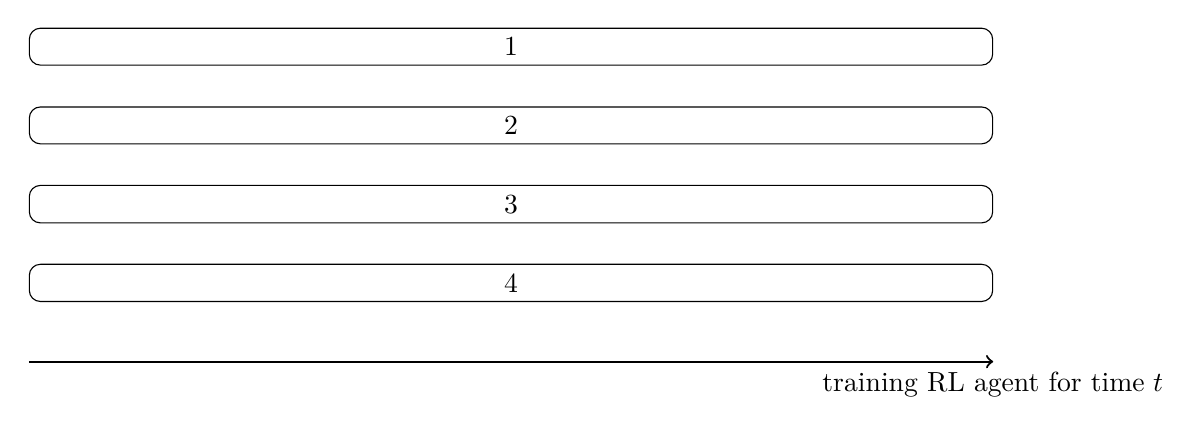
\begin{tikzpicture}[node distance=2.1cm]
%PreProcessing

\node (l1) [activity, text width=12cm] {$\confI{1}$};
\node (l2) [activity, below of=l1, node distance=1cm, text width=12cm] {$\confI{2}$};
\node (l3) [activity, below of=l2, node distance=1cm, text width=12cm] {$\confI{3}$};
\node (l4) [activity, below of=l3, node distance=1cm, text width=12cm] {$\confI{4}$};

\draw[myarrow] ($(l4.west)+(0.0, -1.0)$) -- ($(l4.east)+(0.0, -1.0)$) node[below] {training RL agent for time $t$};

\end{tikzpicture}

\bigskip
\begin{itemize}
	\item Sample many hyperparameter configurations $\confI{i}$ and evaluate them all in parallel
	\pause
	\item Pure exploration on a large population of configurations
	\pause
	\item[$\leadsto$] No dynamic adaptation
\end{itemize}

\end{frame}
%----------------------------------------------------------------------
%----------------------------------------------------------------------
\begin{frame}[c]{Population-based Training \lit{Jaderberg et al. 2017}{https://arxiv.org/pdf/1711.09846.pdf}}

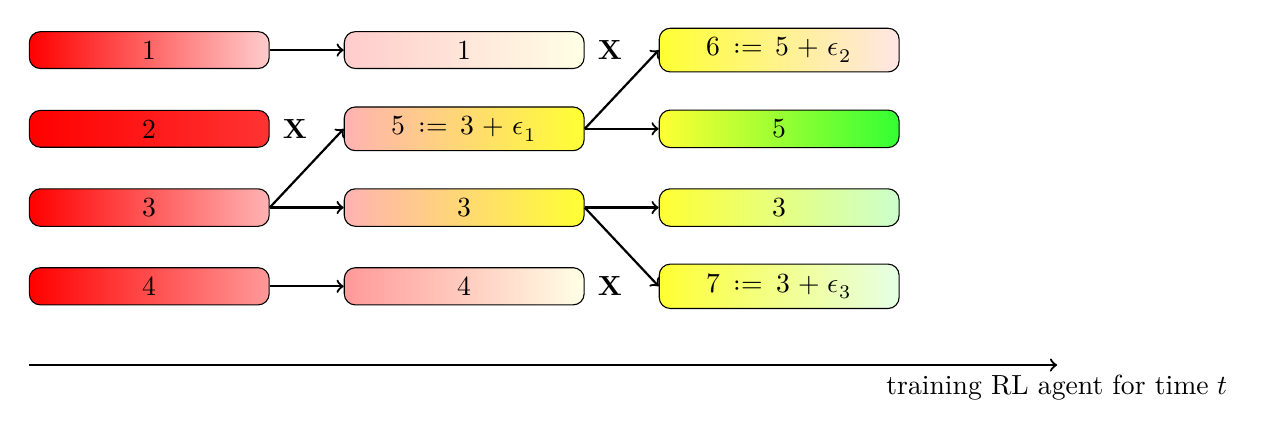
\begin{tikzpicture}[node distance=2.1cm]
%PreProcessing

\node (l1) [activity, left color=red!100, right color=red!20] {$\confI{1}$};
\node (l2) [activity, left color=red!100, right color=red!80, below of=l1, node distance=1cm] {$\confI{2}$};
\node (l3) [activity, left color=red!100, right color=red!30, below of=l2, node distance=1cm] {$\confI{3}$};
\node (l4) [activity, left color=red!100, right color=red!40, below of=l3, node distance=1cm] {$\confI{4}$};

\draw[myarrow] ($(l4.west)+(0.0, -1.0)$) -- ($(l4.east)+(10.0, -1.0)$) node[below] {training RL agent for time $t$};

\pause

\node (l12) [activity, right of=l1, left color=red!20, right color=yellow!10, node distance=4cm] {$\confI{1}$};
\node (l22X) [right of=l2, node distance=1.85cm]{\textbf{X}};
\node (l22) [activity, left color=red!30, right color=yellow!80, right of=l2, node distance=4cm]{$\confI{5} := \confI{3} + \epsilon_1$};
\node (l32) [activity, left color=red!30, right color=yellow!80, right of=l3, node distance=4cm] {$\confI{3}$};
\node (l42) [activity, left color=red!40, right color=yellow!10, right of=l4, node distance=4cm] {$\confI{4}$};

\draw[myarrow] (l1.east) -- (l12.west);
\draw[myarrow] (l3.east) -- (l22.west);
\draw[myarrow] (l3.east) -- (l32.west);
\draw[myarrow] (l4.east) -- (l42.west);

\pause

\node (l13X) [right of=l12, node distance=1.85cm]{\textbf{X}};
\node (l13) [activity, left color=yellow!80, right color=red!10, right of=l12, node distance=4cm] {$\confI{6} := \confI{5} + \epsilon_2$};
\node (l23) [activity, left color=yellow!80, right color=green!80, right of=l22, node distance=4cm]{$\confI{5}$};
\node (l33) [activity, left color=yellow!80, right color=green!20, right of=l32, node distance=4cm] {$\confI{3}$};
\node (l43X) [right of=l42, node distance=1.85cm]{\textbf{X}};
\node (l43) [activity, left color=yellow!80, right color=green!10, right of=l42, node distance=4cm] {$\confI{7} := \confI{3} + \epsilon_3$};

\draw[myarrow] (l22.east) -- (l13.west);
\draw[myarrow] (l22.east) -- (l23.west);
\draw[myarrow] (l32.east) -- (l33.west);
\draw[myarrow] (l32.east) -- (l43.west);

\end{tikzpicture}

\begin{itemize}
	\item The color indicates the performance over time
	\item \textbf{X} indicates the termination of an RL agent training
\end{itemize}

\end{frame}
%----------------------------------------------------------------------
%----------------------------------------------------------------------
\begin{frame}[c]{Population-based Training \lit{Jaderberg et al. 2017}{https://arxiv.org/pdf/1711.09846.pdf} \lit{Liang et al. 2020}{https://arxiv.org/pdf/2002.04225.pdf}}

General workflow of PBT:

\begin{enumerate}
	\item Sample initial population
	\begin{itemize}
		\item Each population member is a combination of hyperparameter setting $\conf$ and (partially trained) model
	\end{itemize}
	\pause
	\item Train population for a bit 
	\pause
	\item Tournament selection to drop poorly performing population members
	\pause
	\item Use mutation (and cross-over) to generate off-springs
	\begin{itemize}
		\item Change the hyperparameter settings, but inherits the partially trained model (+ pertubation)
	\end{itemize}
	\pause
	\item[$\leadsto$] New population consists of so-far best performing ones and new off-springs
	\pause
	\item Go to 2.
\end{enumerate}

\pause
See \lit{Deepmind Blog}{https://deepmind.com/blog/article/population-based-training-neural-networks} for a nice animation

\end{frame}
%----------------------------------------------------------------------
%----------------------------------------------------------------------
\begin{frame}[c]{Properties of Population-based Training (PBT)}

\begin{itemize}
	\item PBT returns an already trained model (e.g., DNN or RL policy)
	\bigskip
	\pause
	\item PBT uses evolutionary computing to determine well-performing hyperparameter settings
	\bigskip
	\pause
	\item Hyperparameter settings changes while training the agent
	\bigskip
	\pause
	\item Since each population member (i.e., model) can be trained independently,\\ PBT can be efficiently parallelized
	\begin{itemize}
		\item[$\leadsto$] Drawback: requires substantial parallel compute resources
	\end{itemize}
\end{itemize}

\end{frame}
%----------------------------------------------------------------------

\end{document}
